\documentclass[a4paper]{article}
\usepackage[UTF8]{ctex}
\usepackage{geometry}
\usepackage{graphicx}
\usepackage{url}
\usepackage{multirow}
\usepackage{array}
\usepackage{booktabs}
\usepackage{url}
\usepackage{enumitem}
\usepackage{graphicx}
\usepackage{float}
\usepackage{amssymb}
\usepackage{amsmath}
\usepackage{subfig}
\usepackage{longtable}
\usepackage{pifont}
\usepackage{color}

\allowdisplaybreaks

\geometry{a4paper, scale=0.78}

\usepackage{tikz}
\newcommand*{\circled}[1]{\lower.7ex\hbox{\tikz\draw (0pt, 0pt)%
    circle (.5em) node {\makebox[1em][c]{\small #1}};}}
    

% \begin{figure}[H]
%     \centering
%     \includegraphics[width=.55\textwidth]{E.png}
%     \caption{矩阵与列向量的乘法}
%     \label{fig:my_label_1}
% \end{figure}

% \left\{
% \begin{array}{ll}
%       x+2x+z=2 & \\
%       3x+8y+z=12 & \\
%       4y+z=2
% \end{array}
% \right.

% \begin{enumerate}[itemindent = 1em, itemsep = 0.4pt, parsep=0.5pt, topsep = 0.5pt]

% \end{enumerate}

%\stackrel{a}{\longrightarrow}

%\underbrace{}_{} %下括号

%\tableofcontents %目录,并且目录页不记录页码
% \tableofcontents
% \newpage
% \setcounter{page}{1} %new page
% \clearpage

\title{Confronting Partition Function}
\author{Chen Gong}
\date{06 March 2020}

\begin{document}
\maketitle
%\pagestyle{empty}
\tableofcontents
\newpage
%\pagestyle{fancy}
\setcounter{page}{1} %new page
\clearpage

\section{Background}
\subsection{直面配分函数的来源}
在概率图模型中,所有的问题基本上都是这三个问题组成的:模型表示(Representation);学习(Learning);推断(Inference)。而Inference中,有精确推断和近似推断(Variational Inference和MCMC)。在之前我们Restricted Boltzmann Machine对模型表示和推断的问题作出了详细的推导,而学习问题当时没有进行推导,这个问题保留到了现在。

在前面的Restricted Boltzmann Machine问题中,我们对随机变量的联合概率建模,并利用势函数等于Boltzmann Distribution的形式来表示变量的联合概率密度函数:
$$
P(X) = \frac{1}{Z} \prod_{i=1}^k \phi_i (x_{c_i}),\quad \phi_i (x_{c_i}) = \exp \left\{ -\mathrm{E}(x_{c_i}) \right\}
$$

其中,能量函数$\mathrm{E}(x)$的参数需要通过从样本中Learning来得到。如果是在有向图模型中,这个联合概率很容易被写成因式分解的形式,但是在无向图中没有top排序的形式。所以,只能根据Markov性质,来将联合概率分布写成最大团的势函数相乘的形式。\textbf{而大家观察一下无向图模型中,就可以发现,局部没有表现为一个概率,而整体才表现出一个概率。}

回想Restricted Boltzmann Machine,很容易发现,实际上\textbf{势函数$\phi_i(\cdot)$的表示形式比较的简单,而配分函数$Z$很不好求。}在求解的过程中,我们无法避免对$Z$的处理,所以叫“直面配分函数”,这个章名字的来由是有点奇怪,而另一种叫法“遭遇配分函数”也是一个意思。

\subsection{求解符号说明}
假设随机变量$X$为$p$维的,即为$X\in \mathbb{R}^p$,而假设每一个维度是0/1分布.所以,$X\in \{0,1\}^p$。随机变量的联合概率分布为:
\begin{equation}
    P(X;\theta) = \frac{1}{Z(\theta)}\hat{P}(X;\theta)
\end{equation}
其中,$\hat{P}(X;\theta)$代表势函数的积,$Z(\theta)= \int \hat{P}(X;\theta)dX$,给定的数据集为$\{x_i\}_{i=1}^N$,其中$x_i^{(j)}$代表第$i$个数据的第$j$维。
\section{极大似然估计法(Maximum Likelihood Estimation)}
\begin{equation}
    \begin{split}
        \hat{\theta} = & \arg\max_{\theta} P(X;\theta) = \arg\max_{\theta} \prod_{i=1}^N \frac{1}{Z(\theta)}\hat{P}(x_i;\theta) \\
        = & \arg\max_{\theta} \prod_{i=1}^N \frac{1}{Z(\theta)}\hat{P}(x_i;\theta) \\
        = & \arg\max_{\theta} \log \prod_{i=1}^N \frac{1}{Z(\theta)}\hat{P}(x_i;\theta) \\
        = & \arg\max_{\theta} \sum_{i=1}^N \log  \frac{1}{Z(\theta)}\hat{P}(x_i;\theta) = \arg\max_{\theta} \sum_{i=1}^N \left[\log \hat{P}(x_i;\theta) - \log Z(\theta) \right]
    \end{split}
\end{equation}

其中,$\log Z(\theta)$和$i$没有关系。所以,$\sum_{i=1}^N \log Z(\theta) = N \log Z(\theta)$。而最大化问题和常数项系数没有太大的关系,所以,将整个等式除以$N$。
\begin{equation}
    \hat{\theta} = \arg\max_{\theta}\underbrace{\frac{1}{N} \sum_{i=1}^N \log \hat{P}(x_i;\theta) - \log Z(\theta)}_{\mathrm{target\ function}}
\end{equation}

下一步,则是求梯度,利用梯度上升法来求解参数,令:
$$
\mathcal{L}(\theta) = \frac{1}{N} \sum_{i=1}^N \log \hat{P}(x_i;\theta) - \log Z(\theta)
$$
而梯度为:
\begin{equation}
    \nabla_\theta \mathcal{L}(\theta) = \frac{1}{N} \sum_{i=1}^N \log \nabla_\theta \hat{P}(x_i;\theta) -\nabla_\theta \log Z(\theta)
\end{equation}
因为,$\hat{P}(x_i;\theta)$是势函数的乘积,势函数的形式一般假设为Boltzmann分布,导数比较简单。而主要是$\nabla_\theta \log Z(\theta)$比较难求。那么这一项怎么求呢?
\begin{equation}
    \begin{split}
       \nabla_\theta \log Z(\theta) = \frac{1}{Z(\theta)} \nabla_\theta Z(\theta) 
    \end{split}
\end{equation}
这里,遇到了一个问题$\frac{1}{Z(\theta)}$,求不出来。那么,根据等式(1),可以得到$Z(\theta) = \frac{\hat{P}(X;\theta)}{P(X;\theta)} = \int \hat{P}(X;\theta) dX$。看到这有很多同学就受不了了,我也是其中一个。你不是要求$P(X;\theta)$吗?怎么又用起来了,这里是这样的,我们采用的是梯度上升的迭代方法,$P(X;\theta^{(t+1)})$的具体形式我们不知道。但是$\theta^{(t)}$是知道的,可以利用$P(X;\theta^{(t)})$这个分布来对$t+1$时刻的梯度方向进行近似求解。然后,下一步的替换有点Initutive,主要的想法\textbf{是$Z(\theta)$求不出来,那么就造一个和$P(X;\theta)$相关的期望,通过在$P(X;\theta)$中采样就可以近似处理这个问题}。那么:
\begin{equation}
    \begin{split}
       \nabla_\theta \log Z(\theta) = & \frac{1}{Z(\theta)} \nabla_\theta Z(\theta) \\
       = & \frac{1}{Z(\theta)} \nabla_\theta \int \hat{P}(X;\theta) dX \\
       = & \frac{1}{Z(\theta)} \int \nabla_\theta  \hat{P}(X;\theta) dX \\
       = & \int  \frac{1}{Z(\theta)}  \nabla_\theta \hat{P}(X;\theta) dX \\
       = & \int  \frac{P(X;\theta)}{\hat{P}(X;\theta)}  \nabla_\theta \hat{P}(X;\theta) dX \\
       = & \int P(X;\theta)  \nabla_\theta \log \hat{P}(X;\theta) dX \\
       = & \mathbb{E}_{P(X;\theta)} [\nabla_\theta \log \hat{P}(X;\theta)]
    \end{split}
\end{equation}

其实,大家学到这有这种感觉,积分很多时候都被看成是期望。对于复杂的积分(无向图中的配分函数$Z$积分求不出来),用期望的思路来从分布中采样来求得,这是一个很常见的思路。而期望可以使用MCMC等方法,从分布中进行采样来求得。

这样,我们就可以求得近似梯度,一步步的求解出近似的最优$\hat{\theta}$。
\subsection{小结}
本小节,我们介绍了无向图模型中Learning问题,在利用极大似然估计进行求解的过程中,将面临着配分函数求解不出来的问题。所以,要直面配分函数,我们的思路是通过在未知分布中采样来求解近似梯度,从而通过梯度上升的方法来求得近似的最优参数。下一小节,我们会详细的梳理一下。

\section{随机极大似然(Stochastic Maximum Likelihood)}
其实,我觉得这种是对近似梯度的一个较为详细的解读,这一章看课程还是听有点绕的。我希望可以把思路理一理来帮助大家进行理解。
\subsection{损失函数梯度优化}
在上一节中,我们定义了求解的目标为:
\begin{equation}
  \left\{
    \begin{array}{ll}
      \hat{\theta} = \arg\max_\theta \mathcal{L}(\theta) & \\
      \mathcal{L}(\theta) = \frac{1}{N} \sum_{i=1}^N \log \hat{P}(x_i;\theta) - \log Z(\theta) & \\
    \end{array}
  \right.  
\end{equation}
我们将采用梯度上升法来求解最优参数,梯度公式为:
\begin{equation}
    \nabla_\theta \mathcal{L}(\theta) = \frac{1}{N} \sum_{i=1}^N \nabla_\theta \log \hat{P}(x_i;\theta) - \mathbb{E}_{P(X;\theta)}[\nabla_\theta \log \hat{P}(X;\theta)]
\end{equation}
因为,我们假设给定的数据集为$\{x_i\}_{i=1}^N$,如果全部使用就是Batch-Gradient Descent。如果觉得$N$太大了,就从$N$个样本中选取一部分,这就称之为mini-Batch Gradient Descent。

~\\

实际上,$\{x_i\}_{i=1}^N$是来自一个真实的概率分布$P_{\mathrm{data}}$,这个分布具体是什么我们永远都不知道。\textbf{我们所得到的样本都是从这个真实分布中采样的结果。}而从真实分布中采样的结果,也就是我们拿到的样本可以构成了一个经验分布为$\hat{P}_{\mathrm{data}}$。

所以,$ \frac{1}{N} \sum_{i=1}^N \nabla_\theta \log \hat{P}(x_i;\theta)$可以是从真实分布中($P_{\mathrm{data}}$)采样得到的关于势函数乘积的均值。而我们想要求的联合概率分布$P(X;\theta)$,是我们建立的一个模型,\textbf{我们的目标就是利用这个模型,根据从真实分布中采样得到的数据来拟合真实分布,从而实现对其他未知数据的推断,}这个模型被称为$P_{\mathrm{model}}$。那么公式(8)可以被简化为:
\begin{equation}
    \nabla_\theta \mathcal{L}(\theta) = \mathbb{E}_{P_{\mathrm{data}}}[ \nabla_\theta \log \hat{P}(x_i;\theta) ] - \mathbb{E}_{P_{\mathrm{model}}}[\nabla_\theta \log \hat{P}(X;\theta)]
\end{equation}
{\color{red}而极大似然估计的目的就是使真实分布$P_{\mathrm{data}}$和建立的模型$P_{\mathrm{model}}$靠的越近越好。}如何从$P_{\mathrm{model}}$中进行采样呢?因为是梯度上升法,在$t$时刻,想要求$t+1$时刻的参数,那么$\theta^{(t)}$是已知的。即为在$t+1$时刻,$P_{\mathrm{model}}=P(X;\theta^{(t)})$。然后用Gibbs采样法,从$P_{\mathrm{model}}$中采出$m$个样本$\{\hat{x}_i\}_{i=1}^m$,Gibbs采样时MCMC的一种,前面在MCMC那一章有非常详细的分析。

\subsection{梯度分析}
为了使似然函数最大化,采用的是梯度上升法,对参数进行更新。
$$
\theta^{(t+1)} = \theta^{(t)} + \eta \nabla_\theta \mathcal{L}(\theta^{(t)})
$$
然后将(8)中的结果代入就可以得到,梯度上升法的完整表达形式为:
\begin{equation}
    \theta^{(t+1)} = \theta^{(t)} + \eta \left[ \frac{1}{m} \left[ \sum_{i=1}^m \nabla_\theta \log \hat{P}(x_i;\theta)|_{\theta=\theta^{(t)}} \right] - \frac{1}{m} \left[ \sum_{i=1}^m \nabla_\theta \log \hat{P}(\hat{x}_i;\theta)|_{\theta=\theta^{(t)}} \right]
    \right]
\end{equation}
注意:$x_i$是从真实分布中采样得到的样本点,$\hat{x}_i$是指通过Gibbs采样从$P_{\mathrm{model}}=P(X;\theta^{(t)})$中得到的样本。\textbf{这就是Gradient Ascent Based Markov Chain Monte Carol。}

最终当$\theta$收敛时,梯度等于0,则表示得到了最优解。此时,$$ \sum_{i=1}^m \nabla_\theta \log \hat{P}(x_i;\theta)|_{\theta=\theta^{(t)}} =  \sum_{i=1}^m \nabla_\theta \log \hat{P}(\hat{x}_i;\theta)|_{\theta=\theta^{(t)}}$$
可以近似的认为$P_{\mathrm{data}} = P_{\mathrm{model}}$。$P_{\mathrm{data}}$是真实分布,是不知道的,我们只能通过从中采样来得到经验分布。$P_\mathrm{model}$是自定义的假设,希望用这个假设的模型通过对经验分布的学习去逼近真实分布。梯度为零时,这两个分布近似相等,也就达到了我们的目的。

下面我们将对梯度函数进行具体的分析,梯度函数可以分成两部分,第一部分是Postive phase:$\sum_{i=1}^m \nabla_\theta \log \hat{P}(x_i;\theta)|$;第二部分是Negative phase:$\sum_{i=1}^m \nabla_\theta \log \hat{P}(\hat{x}_i;\theta)$。$\theta$的改变会对$P_{\mathrm{model}}$产生影响,\textbf{{\color{red}记住我们的目标是令$P_{\mathrm{data}} = P_{\mathrm{model}}$。}}假设,对$P_{\mathrm{data}}$和$P_{\mathrm{model}}$的采样结果如下所示:
\begin{figure}[H]
    \centering
    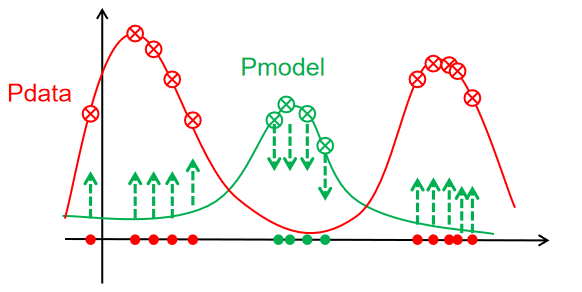
\includegraphics[width=.65\textwidth]{微信图片_20200308152246.png}
    \caption{$P_{\mathrm{data}}$和$P_\mathrm{model}$采样分布图}
    \label{fig:my_label_1}
\end{figure}
其中红色表示从$P_{\mathrm{data}}$中的采样结果$\{x_i\}_{i=1}^m$;绿色表示从$P_{\mathrm{model}}$中的采样结果$\{\hat{x}_i\}_{i=1}^m$。采样都是会趋向于采出概率函数大的区域,如上图所示。因为改变$\theta$,实际上是对$P_{\mathrm{model}}$带来变化。那么对于$P_{\mathrm{data}}$概率值高的地方,自然也希望$P_{\mathrm{model}}$的概率值也高,所以是Postive phase。而对于$P_{\mathrm{model}}$概率值高的地方,是不准确的,我们希望降低它的概率值,这就是Negative Phase。而从另一个方面想,概率密度函数的积分为1,有地方升高就要有地方降低。这就是我对Negative phase和Postive phase的理解。

刚刚将的是对梯度函数的分析。而对目标函数$\mathcal{L}(\theta)$,另外又给出了一个Intuitive的解释,为什么$Z(\theta)$要变少?$Z(\theta) = \int \hat{P}(X;\theta)dX$,这个积分代表的是$\hat{P}(X;\theta)$函数曲线和坐标轴围起来的面积。而$P_{\mathrm{model}}$中的样本称之为“fantasy particle”,是不信任它的,我们信任的是$P_{\mathrm{data}}$真实分布中的样本,所以要把$P_{\mathrm{model}}$中样本对应的概率往下拉。
\subsection{小结}
本小节主要对梯度函数为什么写成这样,做了一个比较直观的解释,个人觉得自己的逻辑思路还算清晰,欢迎各位小伙伴指正。在理解的时候一定要牢记,我们的\textbf{目的是构建一个假设的分布来通过从真实分布中采样得到的经验分布去逼近真实分布}。牢记这一点之后,再去看Negative phase和Postive phase的理解,为什么要拉高$P_{\mathrm{data}}$中的采样结果降低$P_{\mathrm{model}}$中的采样结果,以及为什么要降低$Z(\theta)$等就变得很简单了,对梯度函数中每一项的理解就会清晰很多。

\section{The Problem of Gradient Ascent in MCMC}
\subsection{算法简介}
\noindent When $t+1$:
\begin{enumerate}
    \item Sampling for Postive phase from $P_{\mathrm{data}}$: $\{x_1,x_2,\cdots,x_m\}\sim P_{\mathrm{data}}$,直接从经验分布中采样得到training data。
    \item Sampling for Negative phase from $P_{\mathrm{model}}=P(X;\theta^{(t)})$ ($\theta^{(t)}$已知): $\{\hat{x}_1,\hat{x}_2,\cdots,\hat{x}_m\}\sim P_{\mathrm{model}}$。需要使用Gibbs采样来实现从$P_{\mathrm{model}}$中采样:
    \begin{enumerate}
        \item 初始化$\hat{x}_i$,这个样本可以从任意分布中采样,比如均匀分布或者标准高斯分布,初始化分布和最后的结果没有关系,可以随意选取。
        \item 构建一条链,在经过一段时间(Mixing time)后,收敛到平稳随机分布,如下图所示:
        \begin{figure}[H]
        \centering
        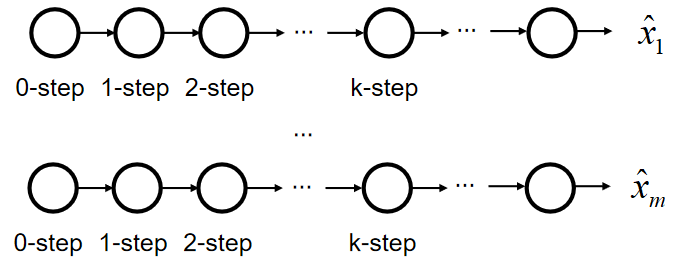
\includegraphics[width=.55\textwidth]{微信图片_20200309153828.png}
        \caption{Gibbs采样示例}
        \label{fig:my_label_1}
        \end{figure}
        我们假设在第$k$步收敛到平稳的状态,之后从平稳分布采一个样本即可。从串行和并行的角度来考虑这个问题,串行角度可以单独使用一条链,待到分布收敛之后,从分布中采$m$次样;并行角度可以使用$m$条链,从每条链的平稳分布中采1次样,这样就能得到$m$个样本点。很显然,并行的方法采样效率更高,但是对内存的消耗也就越大。
    \end{enumerate}
    \item 最后可以得到$t+1$时刻的参数为:
    $$
    \theta^{(t+1)} = \theta^{(t)} + \eta \left[ \frac{1}{m} \left[ \sum_{i=1}^m \nabla_\theta \log \hat{P}(x_i;\theta)|_{\theta=\theta^{(t)}} \right] - \frac{1}{m} \left[ \sum_{i=1}^m \nabla_\theta \log \hat{P}(\hat{x}_i;\theta)|_{\theta=\theta^{(t)}} \right]
    \right]
    $$
\end{enumerate}
\subsection{算法带来的问题}
主要问题就是Mixing time时间太长了,有可能$k \longrightarrow \infty$,这个值实在是太大了。如果,无向图比较简单还好,如果无向图模型过于复杂的话,MCMC很难知道什么时候会到达平稳状态。于是,需要想想别的办法。

\subsection{对比散度(Contrastive Divergence)}
对比散度(Contrastive Divergence)是Hinton在2000年提出来的大作,核心目的是:\textbf{{\color{red}通过寻找合适的初始值来缩短收敛到平稳分布的时间(Mixing time)}}。CD在之前的Gradient Ascent in MCMC上只做出了一点点的改动。

之前,Gibbs采样的初始值是从任意分布中进行采样得到的,我们想找一个合适的初始值,一开始就靠近真实分布,这样就可以压缩Mixing time了。

那么,如何来实现这呢?做法就是从training data中直接采样,这样的效果非常的好。也就是令Gibbs采样的初始值直接等于training data的值:
$$
\hat{x}_1=x_1,\quad \hat{x}_2=x_2,\cdots, \hat{x}_m=x_m
$$
所以,Mixing time可以被大大缩短,称之为CD-K算法。k是可以自己控制的,表示更新k次以后就从分布中进行采样,这里的k是几都可以,而且更新k次以后也不需要一定达到平稳分布。注意,这里的一个step,表示从每一个维度都进行采样后得到一个完整的样本,和样本的维数有关。得到一个样本,$m$维就需要采$m$次。

\subsection{小结}
本小节首先是完整的描述了Gradient Ascent in MCMC,然后讲述了这个算法的确点:收敛所需时间太长了,在模型复杂的情况下没法用。为了压缩到达收敛的时间,然后,描述了Hinton的解决方法,“K-Contrastive Divergence”算法的具体做法,和Gradient Ascent in MCMC唯一的区别即为用training data来代替Gibbs采样的初始值。

\section{The Name of Contrastive Divergence}
第4节中,我们介绍了Contrastive Divergence,主要目的是为了缩短mixing time,其中$K-CD$代表的是不管到不到平稳分布,只执行$K$步转移,就从分布中进行采样。那么,为什么叫对比散度呢?和之前学习的KL Divergence有什么区别和联系呢?

那么,我们对极大似然估计的过程,做一些变换:
\begin{equation}
    \begin{split}
        \hat{\theta} = & \arg\max_{\theta} \frac{1}{N} \sum_{i=1}^N \log P(x_i;\theta) \\
        = & \arg\max_{\theta} \mathbb{E}_{P_{\mathrm{data}}}[ \log P(x_i;\theta)] \\
    \end{split}
\end{equation}
其中,$P(x_i;\theta)$是$P_{\mathrm{model}}$,所有有:
\begin{equation}
\begin{split}
    \hat{\theta}
    = & \arg\max_{\theta} \mathbb{E}_{P_{\mathrm{data}}}[ \log P_{\mathrm{model}}]
    = \arg\max_{\theta} \int P_{\mathrm{data}} \log P_{\mathrm{model}} dx
\end{split}
\end{equation}
而$P_{\mathrm{data}}$和$\theta$之间并没有任何关联,所以添加和$P_{\mathrm{data}}$相关的项,对整体结果没有影响。那么,紧接着公式(12)很显然可以得到:
\begin{equation}
    \begin{split}
        \hat{\theta} = & \arg\max_{\theta} \int P_{\mathrm{data}} \log P_{\mathrm{model}} dx - P_{\mathrm{data}}  \log P_{\mathrm{data}} dx \\
        = & \arg\max_{\theta} \int P_{\mathrm{data}} \log \frac{P_{\mathrm{model}}}{P_{\mathrm{data}}} \\
        = & \arg\max_{\theta} -\mathrm{KL}(P_{\mathrm{data}}||P_{\mathrm{model}}) \\
        = & \arg\min_{\theta} \mathrm{KL}(P_{\mathrm{data}}||P_{\mathrm{model}})
    \end{split}
\end{equation}
这样,我们就再次证明了极大似然估计的目的就是使真实分布与建模分布越靠近越好,靠近的程度用KL散度来衡量,这样就建立KL散度和极大似然估计的联系。总结一下为:
$$
\hat{\theta} = \arg\max_\theta \mathcal{L}(\theta) =  \arg\min_{\theta} \mathrm{KL}(P_{\mathrm{data}}||P_{\mathrm{model}})
$$

~\\

看到上面的公式表达,结合之前的分析,用MCMC从$P_{\mathrm{model}}$中采样时一件很困难的事情(到达平稳分布所需时间太长)。而K-CD的想法是,转移$K$次,到不到平稳分布都不管了,之前从第$K$步转移的分布中进行采样。

在K-CD中,使用的是training data为Gibbs采样的初始值,记为$P^{(0)}$;假设模型很复杂,转移到平稳分布$P_{\mathrm{model}}$所需的时间太长为,记为$P^{(\infty)}$;而实际上,是从第K次转移中就进行采样,记为$P^{(k)}$;那么我们将目标函数做了一个改变:
\begin{equation}
    \mathrm{KL}(P^{(0)}||P^{(\infty)}) \Longrightarrow  \mathrm{KL}(P^{(0)}||P^{(k)})
\end{equation}
而$\mathrm{KL}(P^{(0)}||P^{(k)})$可以等价的写为:
\begin{equation}
    \mathrm{KL}(P^{(0)}||P^{(k)}) = \mathrm{KL}(P^{(0)}||P^{(\infty)}) - \mathrm{KL}(P^{(k)}||P^{(\infty)})
\end{equation}
这个公式(15)就被定义为“Contrastive Divergence”,这时计算出来的是一个近似的梯度,因为$\hat{x}_i$是来自于$P^{(k)}$,而不是$P^{(\infty)}$,这个算的上是系统误差了。公式完整表达如下所示:
\begin{equation}
    \hat{\theta} = \underbrace{\mathrm{KL}(P^{(0)}||P^{(\infty)}) - \mathrm{KL}(P^{(k)}||P^{(\infty)})}_{\mathrm{Contrastive\ Divergence}} = \eta \left[ \frac{1}{m} \left[ \sum_{i=1}^m \nabla_\theta \log \hat{P}(x_i;\theta)|_{\theta=\theta^{(t)}} \right] - \frac{1}{m} \left[ \sum_{i=1}^m \nabla_\theta \log \hat{P}(\hat{x}_i;\theta)|_{\theta=\theta^{(t)}} \right]
    \right]
\end{equation}

整个算法为CD-Learning,变化之前原始的版本是Maximum Likelihood Learning。

\subsection{小结}
这一小节中,通过将Likelihood变化成KL散度的形式,我们看到了损失函数和散度的关系。然后,通过变换了解了Contrastive Divergence算法中Divergence的来源,实际上就是KL散度的一个变形,只不过是对一个中间分布求KL散度,而不是对最后的精准分布求。我感觉这个算法的近似尺度有点大,但是神奇的很work。看到这里,不少同学会觉得有点抽象,下面我们就用之前遗留下来的RBM的学习问题为基础来讲述CD算法在其中的运用。

\section{Restricted Boltzmann Machine Learning}
之前的描述是站在一个较高的高度来看无向图模型中Learning问题是如何解决的,接下来就以RBM中的Learning为例,来看看CD算法是如何工作的。RBM的Learning问题中,由于Gibbs Sampling
收敛所需时间过长的问题,所以采用基于CD的高效的Gibbs采样。在之前的描述中,$\hat{P}(X)$中都是observed的节点,没有hidden节点,这里和RBM有点不太一样,不过基本都是一样的。

\subsection{Restricted Boltzmann Machine模型描述}
这里只做简要的描述,具体请看之前有关RBM的详细描述。这里只做简要概述,RBM概率图模型如下所示:
\begin{figure}[H]
    \centering
    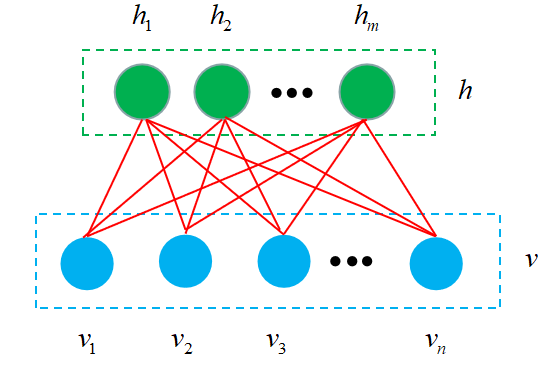
\includegraphics[width=.45\textwidth]{微信图片_20200311150228.png}
    \caption{Restricted Boltzmann Machine概率图模型}
    \label{fig:my_label_1}
\end{figure}
公式化表达如下所示:
\begin{equation}
    X = \begin{bmatrix}
    x_1 \\
    x_2 \\
    \vdots \\
    x_p
    \end{bmatrix}
    = 
    \begin{bmatrix}
    h \\
    v
    \end{bmatrix}
    ,\quad
    h = 
    \begin{bmatrix}
    h_1 \\
    h_2\\
    \vdots \\
    h_m
    \end{bmatrix}
    ,\quad
    v = 
    \begin{bmatrix}
    v_1 \\
    v_2\\
    \vdots \\
    v_n
    \end{bmatrix},\quad
    w = [w_ij]_{m\times n}, \quad
    \alpha = 
    \begin{bmatrix}
    \alpha_1 \\
    \alpha_2\\
    \vdots \\
    \alpha_n
    \end{bmatrix},\quad
    \beta = 
    \begin{bmatrix}
    \beta_1 \\
    \beta_2\\
    \vdots \\
    \beta_m
    \end{bmatrix},\quad
\end{equation}
\begin{equation}
    \begin{split}
        P(X) 
        = &  \frac{1}{Z} \exp (-\mathrm{E}(v,h)) \\
    \mathrm{E}(v,h) = & - h^T w v + \alpha^T v + \beta^T h \\
    = & - \left( \sum_{i=1}^m \sum_{j=1}^n h_iw_{ij}v_i + \sum_{j=1}^n \alpha_j v_j + \sum_{i=1}^m \beta_i h_i 
    \right)
    \end{split}
\end{equation}
其中,$\alpha$和$\beta$都是一样的,我们重点的关注对象是关于$w_{ij}$的求解,这个的求解难度大一点。求解过程分为两部分,求Likelihood Function和Log Likelihood Gradient。

\subsection{Likelihood Function}
假定training set为observed data set,$v\in S$,$|S|=N$。那么Likelihood function的形式很简单,可以表示为:
\begin{equation}
    \frac{1}{N} \sum_{v\in S} \log P(v)
\end{equation}
\subsection{Log Likelihood Gradient}
Likelihood Function的梯度求解为:
\begin{equation}
   \frac{1}{N}  \frac{\partial}{\partial \theta} \sum_{v\in S} \log P(v)
\end{equation}
\begin{equation}
    \log P(v) = \log \sum_h P(h,v) = \log \sum_h \frac{1}{Z} \exp\{-\mathbb{E}(h,v)\}
\end{equation}
而归一化因子$Z$的表达式即为:$Z = \sum_h \sum_v \exp\{-\mathbb{E}(h,v)\}$,所以:
\begin{equation}
    \log P(v) = \underbrace{\sum_h \exp\{-\mathbb{E}(h,v)\}}_{\circled{1}} - \underbrace{\sum_h \sum_v \exp\{-\mathbb{E}(h,v)\}}_{\circled{2}}
\end{equation}
而$\theta = \{w,\alpha,\beta\}$,梯度公式为:
\begin{equation}
    \frac{\partial }{\partial \theta} \log P(v) = \frac{\partial }{\partial \theta} \circled{1} - \frac{\partial }{\partial \theta} \circled{2}
\end{equation}
其中:
\begin{equation}
    \begin{split}
        \frac{\partial }{\partial \theta} \circled{1} = & \frac{\partial }{\partial \theta} \sum_h \exp\{-\mathbb{E}(h,v)\} \\
        = & \frac{-1}{\sum_h \exp\{-\mathbb{E}(h,v)\}} \sum_h \exp\{-\mathbb{E}(h,v)\} \frac{\partial }{\partial \theta} \mathbb{E}(h,v)
    \end{split}
\end{equation}
由于$\sum_h \exp\{-\mathbb{E}(h,v)\} = \exp\{-\mathbb{E}(v)\}$是和$h$无关的项。所以,可以写到$\sum_h$里面,即为:
\begin{equation}
    \begin{split}
        \frac{\partial }{\partial \theta} \circled{1} = & -\sum_h \frac{\exp\{-\mathbb{E}(h,v)\}}{\sum_h \exp\{-\mathbb{E}(h,v)} \frac{\partial }{\partial \theta} \mathbb{E}(h,v) \\
        = & -\sum_h \frac{\frac{1}{Z} \exp\{-\mathbb{E}(h,v)\}}{\frac{1}{Z}\sum_h \exp\{-\mathbb{E}(h,v)} \frac{\partial }{\partial \theta} \mathbb{E}(h,v) \\
        = & -\sum_h \frac{\frac{1}{Z} \exp\{-\mathbb{E}(h,v)\}}{\frac{1}{Z} \exp\{-\mathbb{E}(v)} \frac{\partial }{\partial \theta} \mathbb{E}(h,v) \\
        = & -\sum_h \frac{P(h,v)}{P(v)} \frac{\partial }{\partial \theta} \mathbb{E}(h,v) \\
        = & -\sum_h P(h|v) \frac{\partial }{\partial \theta} \mathbb{E}(h,v) \\
    \end{split}
\end{equation}
同样,$\sum_h \sum_v \exp\{-\mathbb{E}(h,v)\}$和$h,v$都没有关系,所以,
\begin{equation}
    \begin{split}
        \frac{\partial }{\partial \theta} \circled{2} = & \frac{\partial }{\partial \theta}  \sum_h \sum_v \exp\{-\mathbb{E}(h,v)\} \\
        = & \frac{-1}{\sum_h \sum_v \exp\{-\mathbb{E}(h,v)\}} \sum_h \sum_v \exp\{-\mathbb{E}(h,v)\} \frac{\partial }{\partial \theta} \mathbb{E}(h,v) \\
        = & -\sum_h \sum_v \frac{\exp\{-\mathbb{E}(h,v)\}}{\sum_h \sum_v \exp\{-\mathbb{E}(h,v)} \frac{\partial }{\partial \theta} \mathbb{E}(h,v) \\
        = & -\sum_h \sum_v \frac{\exp\{-\mathbb{E}(h,v)\}}{Z} \frac{\partial }{\partial \theta} \mathbb{E}(h,v) \\
        = & -\sum_h \sum_v P(h,v) \frac{\partial }{\partial \theta} \mathbb{E}(h,v) \\
    \end{split}
\end{equation}
综上所述,$\frac{1}{N} \frac{\partial }{\partial \theta} \log P(v)$可以表达为:
\begin{equation}
\begin{split}
    \frac{1}{N} \frac{\partial }{\partial \theta} \log P(v) = & \frac{1}{N} \left( \frac{\partial }{\partial \theta} \circled{1} - \frac{\partial }{\partial \theta} \circled{2} \right)\\
    = &\frac{1}{N} \left( \sum_h \sum_v P(h,v) \frac{\partial }{\partial \theta} \mathbb{E}(h,v) - \sum_h P(h|v) \frac{\partial }{\partial \theta} \mathbb{E}(h,v)\right)
\end{split}
\end{equation}
那么,基于Energy函数的带隐变量的Likelihood Gradient的形式就表达出来了。

\subsection{针对$w$参数的Log Likelihood Gradient}
前面已经说了,$\theta=\{w,\alpha,\beta\}$,其中$\alpha$和$\beta$的求解比较简单,我们主要是求解$w$。
\begin{equation}
    \frac{\partial }{\partial \theta} \log P(v) 
    = \sum_h \sum_v P(h,v) \frac{\partial }{\partial \theta} \mathbb{E}(h,v) - \sum_h P(h|v) \frac{\partial }{\partial \theta} \mathbb{E}(h,v)
\end{equation}
令$\theta = w_{ij}$:
\begin{equation}
    \frac{\partial }{\partial w_{ij}} \log P(v) 
    = \sum_h \sum_v P(h,v) \frac{\partial }{\partial w_{ij}} \mathbb{E}(h,v) - \sum_h P(h|v) \frac{\partial }{\partial w_{ij}} \mathbb{E}(h,v)
\end{equation}
而$\mathrm{E}(v,h) = - h^T w v + \alpha^T v + \beta^T h$,因为$\alpha^T v + \beta^T h$和$w_{ij}$之间没有关系,基本不用看,我们就用$\triangle$来表示。那么,$\mathrm{E}(v,h) = - h^T w v + \triangle$,那么:
$$
 \mathrm{E}(v,h) = - \left( \sum_{i=1}^m \sum_{j=1}^n h_iw_{ij}v_i + \triangle \right)
$$
所以:
\begin{equation}
    \begin{split}
    \frac{\partial }{\partial w_{ij}} \log P(v) 
    = & \sum_h \sum_v P(h,v) (-h_iv_j) - \sum_h P(h|v) (-h_iv_j) \\
    = & \sum_h P(h|v) h_iv_j - \sum_h \sum_v P(h,v)h_iv_j
    \end{split}
\end{equation}
那么,下一步的问题就是如何求解$\sum_h P(h|v)h_iv_j$和$\sum_h \sum_v P(h,v)h_iv_j$。为了简化运算,我们令RBM中每个节点都是0/1分布,即为$y_i,h_i\in \{0,1\}$。
\subsubsection{$P(h|v)$求解}
\begin{equation}
    \begin{split}
        P(h|v)h_iv_j = & \sum_{h_1}\sum_{h_2}\cdots\sum_{h_i}\cdots\sum_{h_m} P(h_1,h_2,\cdots,h_i,\cdots,h_m|v)h_iv_j
    \end{split}
\end{equation}
因为,后面的$h_iv_j$只和$h_i$相关。所以,把$P(h|v)$中除了$h_i$以外所有的项都求和掉,得到的就是边缘概率分布:
\begin{equation}
    P(h|v)h_iv_j = \sum_{h_i} P(h_i|v)h_iv_j
\end{equation}
又因为$h_i \in \{0,1\}$,所以:
\begin{equation}
    \sum_{h_i} P(h_i|v)h_iv_j = P(h_i=0|v)0v_j + P(h_i=1|v)1v_j = P(h_i=1|v)v_j
\end{equation}
而在之前的章节中,我们就已经详细的推导过了:
\begin{equation}
    P(h_i=1|v) = \sigma( h_i(v)) = \sigma(\sum_{j=1}^n w_{ij}v_i + \beta_i)
\end{equation}
我们使用的是梯度上升的思路,所以这里的$\beta_i$和$w_{ij}$都是上一个时刻计算出的,即为:$\beta_i^{(t)}$和$w_{ij}^{(t)}$。那么:
\begin{equation}
\begin{split}
    P(h|v)h_iv_j = & \sigma(\sum_{j=1}^n w_{ij}v_i + \beta_i) v_j \\
\end{split}
\end{equation}
\subsubsection{$P(h,v)$求解}
\begin{equation}
\begin{split}
    P(h,v)h_iv_j = & \sum_h\sum_v P(v)P(h|v) h_iv_j \\
    = & \sum_v P(v) \sum_h P(h|v) h_iv_j
\end{split}
\end{equation}
而$\sum_h P(h|v) h_iv_j$已经计算过了,而下一步则是求解$P(v)$。而根据我们之前求解的结果:
\begin{equation}
\begin{split}
    P(v) = \frac{1}{Z} \exp\left(\alpha^T v + \sum_{i=1}^m \log ( 1+\exp(w_iv+\beta_i)) \right)
\end{split}
\end{equation}
这个计算太复杂了,精确的计算出来太难了,所以我们需要使用MCMC,Gibbs采样的方法来近似求解。

\subsection{CD-K for Restricted Boltzmann Machine}
\begin{equation}
    \begin{split}
    \frac{\partial }{\partial w_{ij}} \log P(v) 
    = & \sum_h P(h_i=1|v) v_j - \sum_v P(v) P(h_i=1,v)v_j
    \end{split}
\end{equation}
其中,$\sum_h P(h_i=1|v) v_j$可以计算出来,可以直接用training set表示;而$\sum_v P(v) P(h_i=1,v)v_j$是intractable,那么我们的主要目标就是求解这个intractable的部分,主要思想是用采样法(CD-K)来解决。CD-K直接以training set为初始值。

实际上,$\sum_v P(v) P(h_i=1,v)v_j$,可以看成是期望$\mathbb{E}_{P(v)}[P(h_i=1,v)v_j]$,那么我们的重点是如何从$P(v)$中进行采样,把采样的结果代入到$P(h_i=1,v)v_j]$中即可。由于,$P(v)$非常的复杂,所以采用基于CD-K的Gibbs采样,$v$的初始值是训练数据集,采样模型如下所示:
\begin{figure}[H]
    \centering
    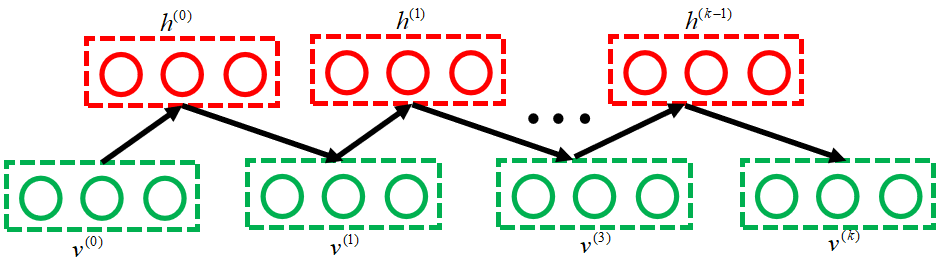
\includegraphics[width=.85\textwidth]{微信图片_20200311212825.png}
    \caption{Gibbs采样示意图}
    \label{fig:my_label_1}
\end{figure}
注意,传统的Gibbs采样时固定是一维一维的采。由于RBM的良好性质,$v$中的节点都是相互独立的,所以可以多个节点一起采,被称之“块Gibbs采样”。这样,$v^{(0)}$是training set,$v^{(k)} \sim P(v)$。这样就可以成功的计算$\sum_v P(v) P(h_i=1,v)v_j$了,那么这个梯度的计算也就搞定了。

~\\

最后,来总结一下CD-K for Restricted Boltzmann Machine:

For each $v\in S$:

\qquad $v^{(0)}\longleftarrow v$;

\qquad For $l=1,2,\cdots,k-1$;

\qquad \qquad For $i=1,2,\cdots,m$: Sampling $h_i^{(l)} \sim P(h_i|v^{(l)})$;

\qquad \qquad For $ j=1,2,\cdots,n$: Sampling $v_j^{(l+1)} \sim P(v|h^{(l)})$; (k-step block Gibbs Sampling);

\qquad For  $i=1,2,\cdots,m;\ j=1,2,\cdots,n$:
$$
\triangle w_{ij} \longleftarrow \triangle w_{ij} + \frac{\partial}{\partial w_{ij}} \log P(v)
$$
$$
\frac{\partial}{\partial w_{ij}} \log P(v) = P(h_i=1|v^{(0)}) v_j^{(0)} - P(h_i=1|v^{(k)})v_j^{(k)}
$$

其中,$P(h_i=1|v^{(0)})$和$P(h_i=1|v^{(k)})$都已经计算出来了。$P(h_i=1|v^{(0)}) v_j^{(0)}$是training set,$v_j^{(k)}$是以training set为起点,经过$K$步后采出来的$N$个样本。根据公式(19),那么最终得到的梯度为:
\begin{equation}
    \frac{1}{N} \sum_{v\in S} \frac{\partial}{\partial w_{ij}} \log P(v) = \frac{1}{N} \triangle w_{ij}
\end{equation}
既然,梯度已经计算出来了,使用梯度上升的方法就可以得到最终的结果了,后面的过程很简单的。

\subsection{小节}
本小节主要是介绍了RBM模型中Learning问题的求解,也是对无向图Learning问题的一个实例。主要问题在求解Likelihood function gradient的过程中,$P(v)$的模型过于复杂,不好进行求解,所以采用基于CD-K的Gibbs采样方法来进行近似。确定了梯度,我们就可以利用梯度上升法愉快的更新了,直到计算中最优值。

\section{总结}
在这一章节中,主要介绍的是无向图中参数Learning的问题。主要思想是对联合概率密度函数求极大似然估计,通过对极大似然函数求梯度来求最优参数。在对配分函数$Z$进行化简的过程中,得到了一个关于$P(X;\theta)$的分布,这个分布过于复杂只能通过MCMC采样的方法来近似。

然后,我们对似然梯度的组成成分进行了分析,似然函数的最终目的是使建立的模型$P_{\mathrm{model}}$和$P_{\mathrm{data}}$靠近。

之后,MCMC由于存在mixing time时间过长的问题,收敛太慢。于是,Hinton提出了,K-Contrastive Divergence (K-CD)算法的具体做法,和MCMC唯一的区别即为用training data来代替Gibbs采样的初始值,而且K-CD算法并不在乎是否收敛,执行K步后直接进行采样。

为了充分的理解CD,我们介绍了CD与KL散度之间的区别和联系,并在其中成功的把Likelihood function转换成了使KL散度最小的问题,这帮助我们进一步的理解了Likelihood Function的作用。

最后,为了具体的理解无向图中的Learning问题,以Restricted Boltzmann Machine问题中的Learning问题为例,来帮助读者加深对前面描述的抽象求解过程的理解。在求解过程中由于$P(v)$的模型过于复杂,不好进行求解,所以采用基于CD-K的Gibbs采样方法来进行近似。确定了梯度,我们就可以利用梯度上升法了。
\end{document}
